\chapter{Discover Selected Approaches}
In this chapter, we will explore some Imitation Learning approaches, that were applied to real robots to get a better practical understanding of the theoretical field. 

% ToDo: End-to-End trained
\section{Paper - Vid2Robot: End-to-end Video-conditioned Policy Learning with Cross-Attention Transformers}

Vid2Robot, a end-to-end video-based learning framework for robots. Given a human or robot video demonstration of a manipulation task and the robot's current visual observations, Vid2Robot directly produces corresponding robot actions in it's own environment. The Demonstration Video can be taken in a different environment or from a different viewpoint. Additionally, Vid2Robot exhibits emergent capabilities, such as successfully transferring observed motions from one object to another (see Figure~\ref{fig:Vid2RobotGeneralization}), and long-horizon composition, thus showcasing its potential for real-world applications.

\begin{figure}[!ht]
	\centering
	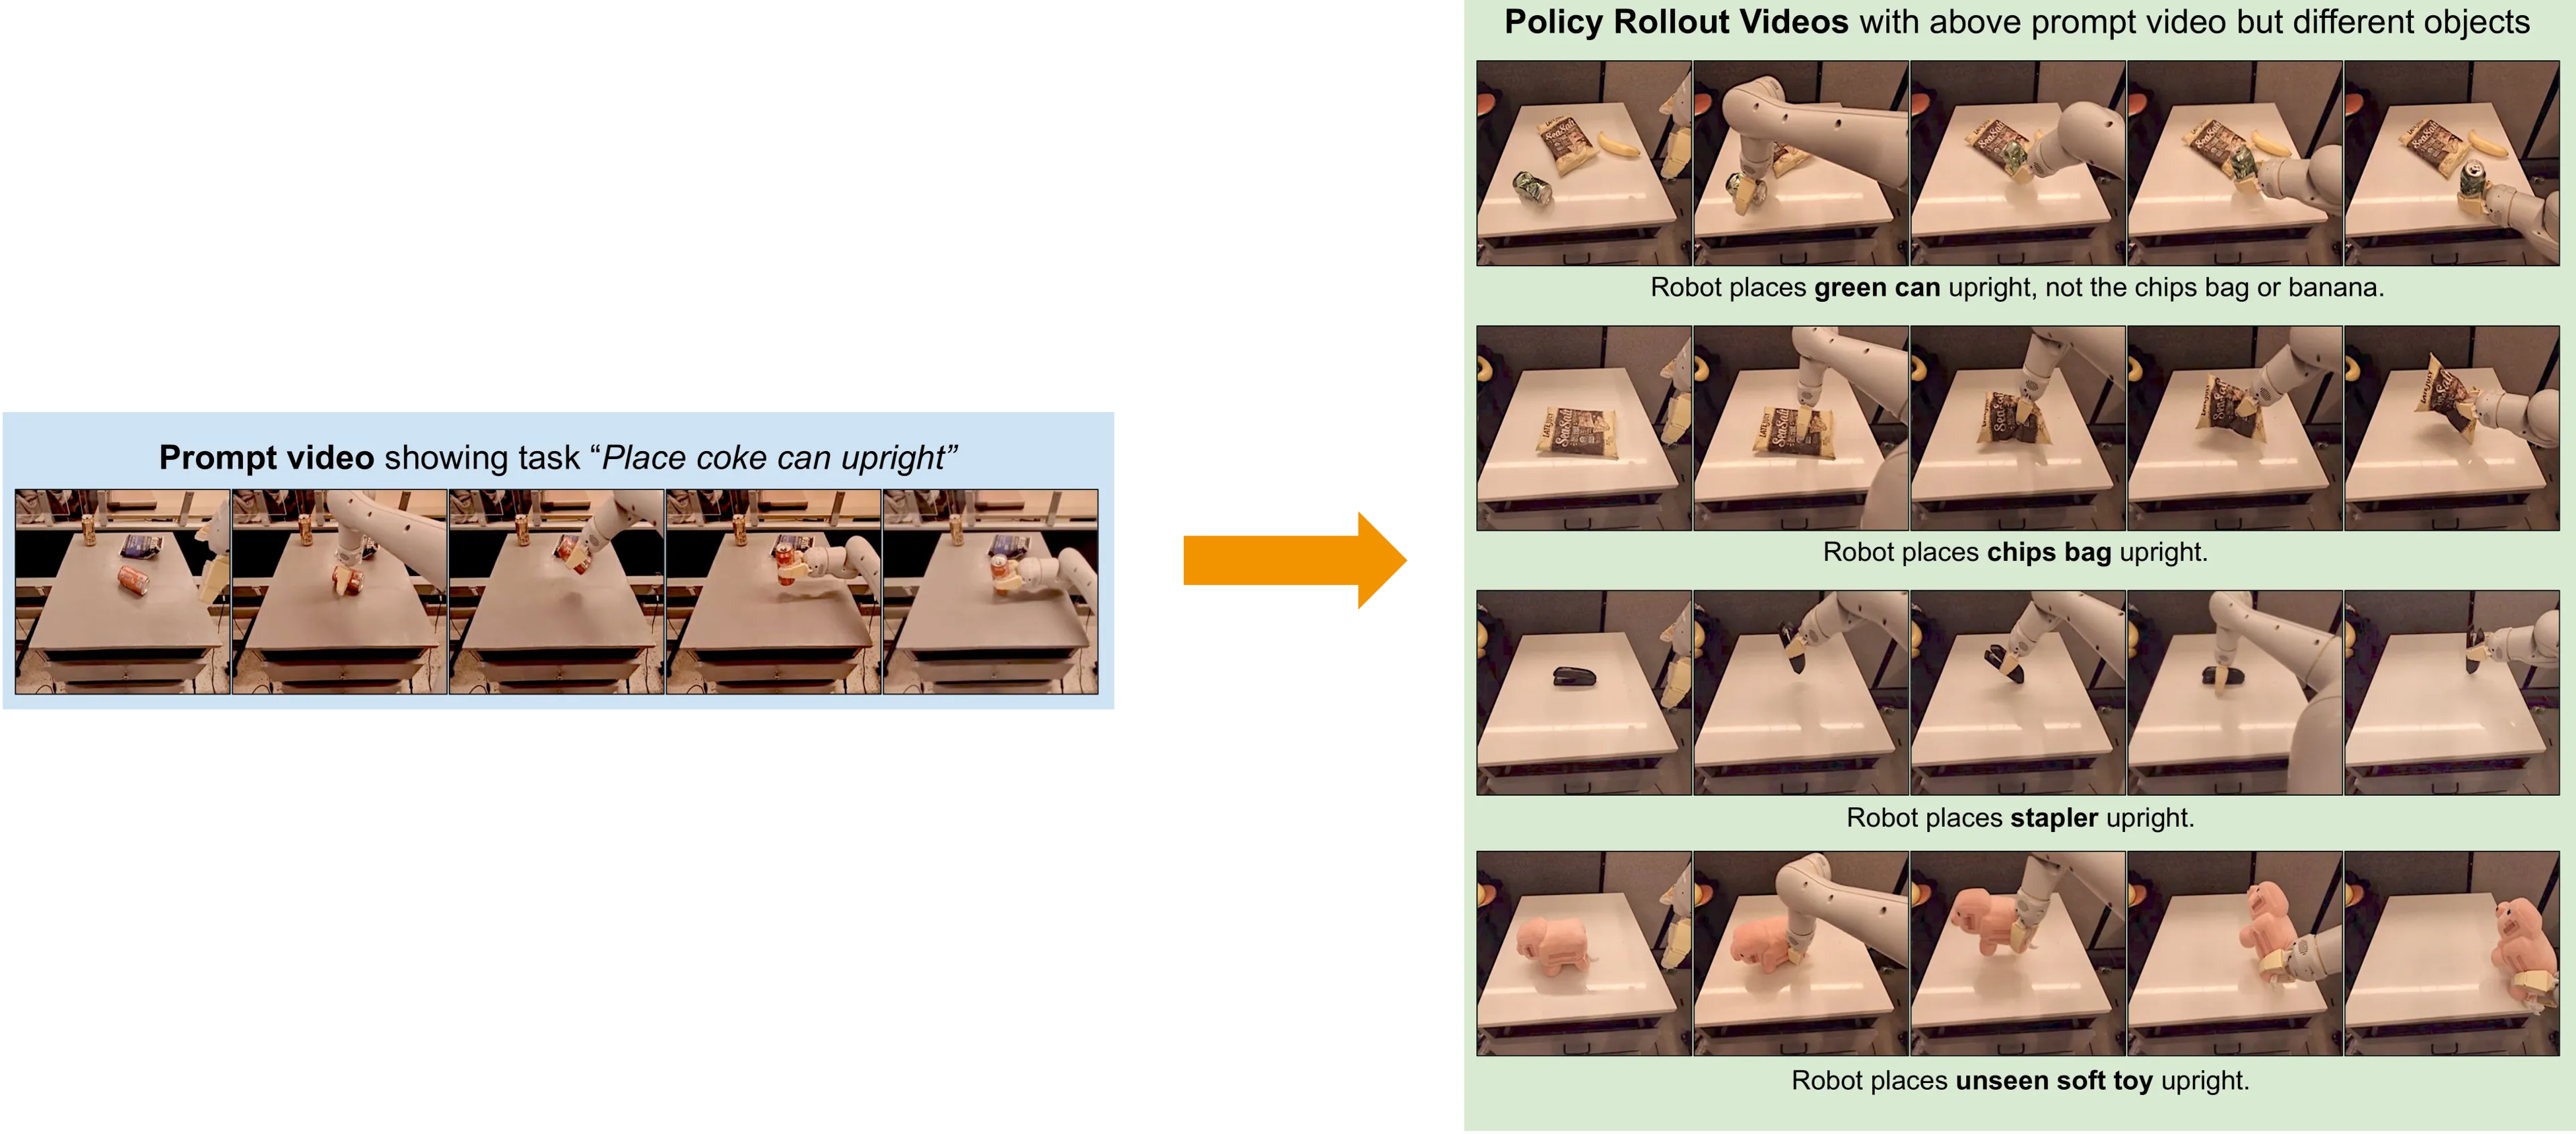
\includegraphics[width=1.0\linewidth]{./chapter8/media/Vid2Robot_Generalization.png}
	\caption[Vid2Robot can transfer observed motions from one object to another]{Vid2Robot can transfer observed motions from one object to another. \cite{?}.}
	\label{fig:Vid2RobotGeneralization}
\end{figure}



\subsection{Architecture}
\begin{figure}[!ht]
	\centering
	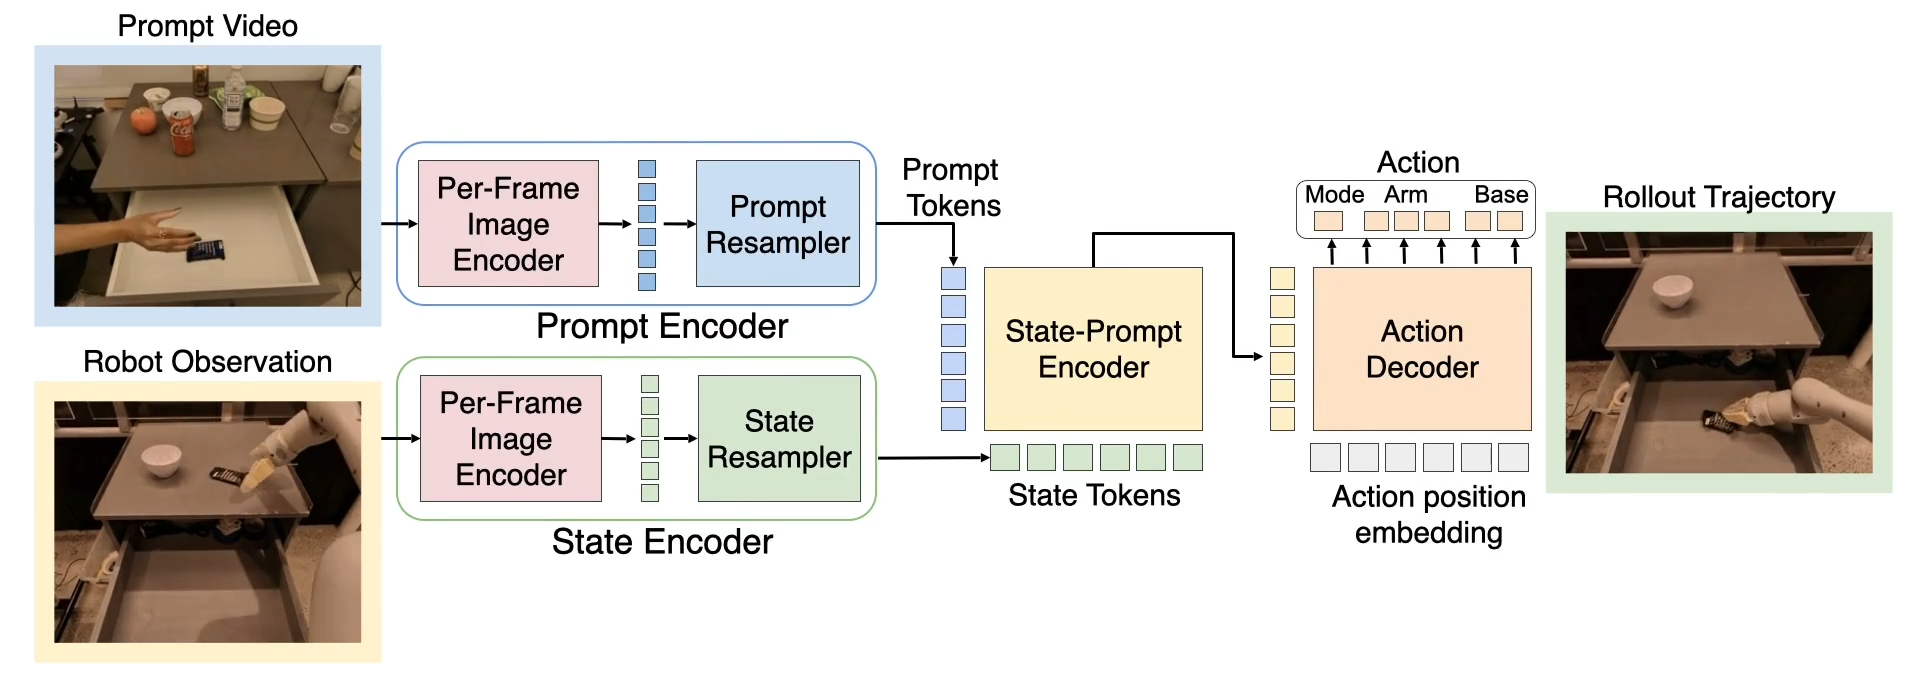
\includegraphics[width=1.0\linewidth]{./chapter8/media/Vid2Robot_Architecture.png}
	\caption[Vid2Robot Architecture]{Vid2Robot Architecture \cite{?}.}
	\label{fig:Vid2RobotArchitecture}
\end{figure}


% The core of Vid2Robot is a cross-attention transformer architecture that effectively fuses information from both the video demonstration and the robot's current observations, enabling it to learn complex manipulation tasks from human or robot demonstrations. 
The policy takes as input the prompt video and the current robot state and outputs robot actions. Vid2Robot consists of four
modules: 
\begin{enumerate}
    \item \textbf{Video Prompt Encoder}
        \begin{itemize}
            \item \textbf{Task:} 
            Encode demonstration video into meaningful representations that capture the essential information about the task being demonstrated.
            \item \textbf{Input:} A human or robot demonstration video of a manipulation task, which should be performed by the robot. 
            \item \textbf{Processing:} 
            Each frame of the demonstration video is first passed through a \texttt{Per-Frame Image Encoder}, which is implemented as a Vision Transformer and capture spatial visual information in each frame. Afterwards, a \texttt{Perceiver Prompt Resampler} aggregates frame tokens over time, reducing the number of tokens while preserving and restructuring temporal information, enabling temporal learning across frames. 
            % \item \textbf{Output:} A set of N tokens of dimension d, which form a compact semantic representation of the demonstration video that can be effectively used to condition the policy.
            \item \textbf{Output:} 
            The Prompt Video Encoder produces a set of d-dimensional \texttt{Prompt Tokens}, which form a compact semantic representation of the demonstration video, capturing \textit{what} needs to be done in the task and \textit{how} to do it. 
            \item \textbf{Purpose:} 
            Represent the demonstrated task goal and motion patterns.
        \end{itemize}
    \item \textbf{Robot State Encoder}
        \begin{itemize}
            \item \textbf{Task:} 
            Encode the robot's current visual observation about objects and the environment into meaningful representations.
            \item \textbf{Input:} The robot's observation, which includes the current and last k robot camera frames.
            \item \textbf{Processing:} 
            The Processing pipeline is the same as in the Prompt Video Encoder, where each frame is first passed through a \texttt{Per-Frame Image Encoder} and then aggregated over time using a \texttt{Perceiver State Resampler}. The weights of the \texttt{Per-Frame Image Encoder} between the Prompt Encoder and State Encoder are shared.
            % , which encourages the model to learn a shared visual representation space for both human and robot videos, thus facilitating better generalization and transfer of learned skills from human demonstrations to robot actions.
            \item \textbf{Output:} 
            Produces \texttt{State Tokens} describing a compact representation of the robot's current visual scene and the objects within it. 
            \item \textbf{Purpose:} 
            Temporal encoding of the robot state, which allows understanding of object motion and robot context
        \end{itemize}
    \item \textbf{State-Prompt Encoder} 
        \begin{itemize}
            \item \textbf{Task:} 
            Align the robot's current view with the demonstrated goal
            % \item fuses the information from the prompt and observation encoders to produce a combined representation.
            \item \textbf{Input:} The State
            \item \textbf{Processing:} 
            Implemented using a Cross-Attention Transformer, with the robot state tokens as queries and the prompt tokens as keys and values. 
            \item \textbf{Output:} 
            Produces \texttt{Prompt-Aware State Tokens}, which are enriched state representations that focus on task-relevant objects or regions of the robot's current observation.
            \item \textbf{Purpose:} 
            Helps the robot to look at the apple in a ``pick apple'' demo.
        \end{itemize}
    \item \textbf{Action Decoder}: decodes the combined representation into robot actions.
        \begin{itemize}
            \item \textbf{Task:} 
            Predict next robot action
            \item \textbf{Input:} The State
            \item \textbf{Processing:} 
            Implemented using a transformer decoder architecture, with fixed action position embeddings as queries, and the prompt-aware state tokens as keys and values. Each output token embedding is projected to 256 dimensions and the action bin with the highest probability is selected.
            \item \textbf{Output:} 
            Multi-dimensional robot action vector, with components for the mode, arm and base. Mode determines whether to terminate the epsidoe, move only the arm, the base or both. Arm describes the gripper pose and the state of the gripper (degree of closedness) and base the displacement and rotation of the robot base.
            \item \textbf{Purpose:} 
            Predicts the robot actions for the next 4 timesteps.
        \end{itemize}
\end{enumerate}
Cross-Attention Transformer layers are used in Perceiver Prompt Resampler, Perceiver State Resampler, State-Prompt Encoder and Action Decoder


\subsection{Training}
To handle the varying lengths of demonstration videos, Vid2Robot samples randomly $N = 16$ frames. The first and last frames are always included to capture the initial and final states of the task, while the other sampled frames are selected randomly and sorted by their temporal order. The frames of the video prompt and robot observation are normalized between 0 to 1, rezized to 224x224 pixels and photometric augmentations like cropping, brightness, contrast, hue and saturation are applied during training.

% To further improve policy performance, we propose auxiliary
% contrastive losses that enhance the alignment between human
% and robot video representations.


\begin{figure}[!ht]
	\centering
	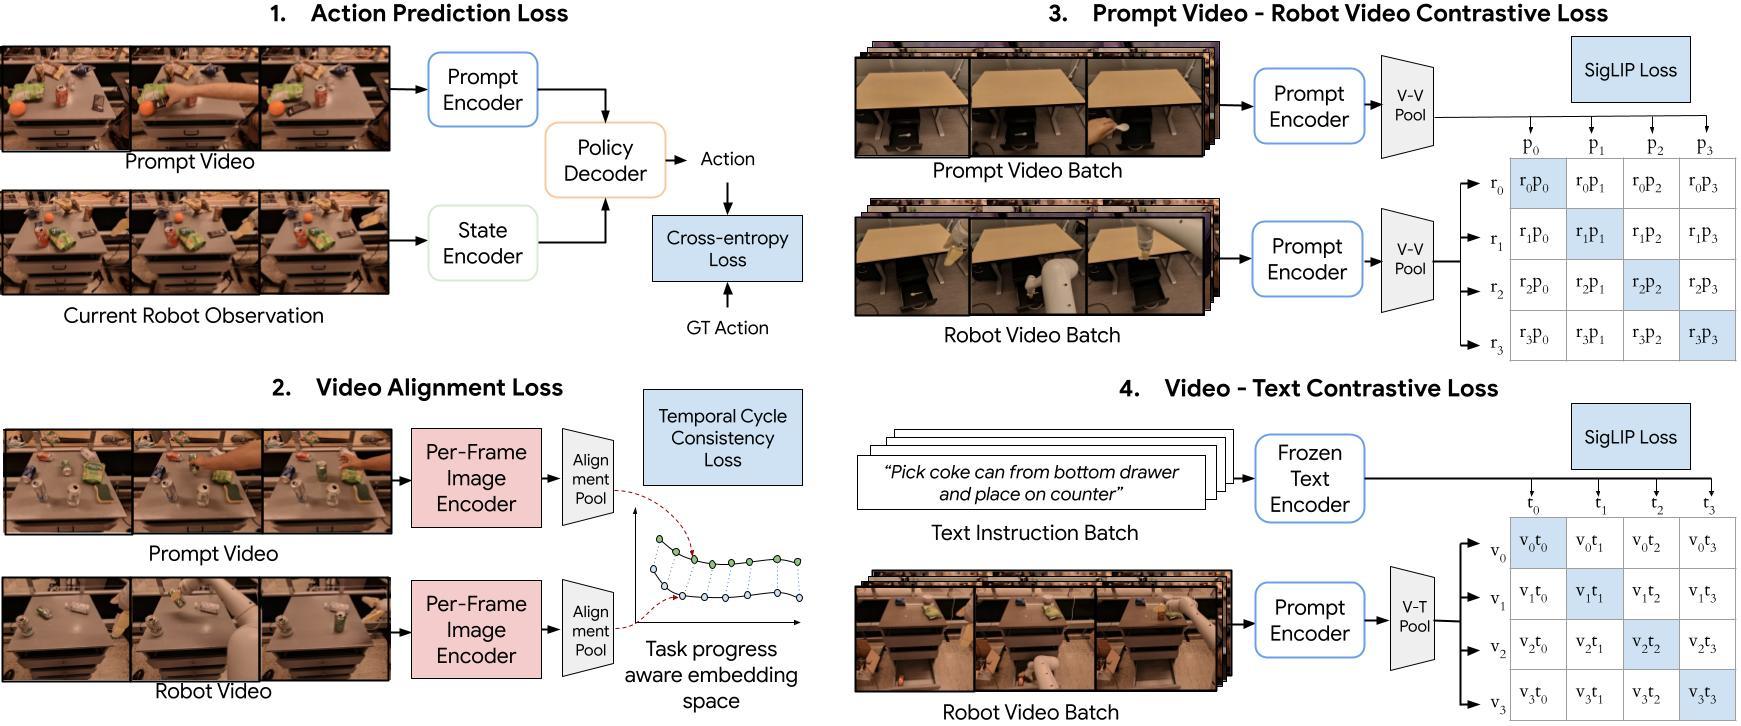
\includegraphics[width=1.0\linewidth]{./chapter8/media/Vid2Robot_Loss.png}
	\caption[Vid2Robot Loss]{Vid2Robot Loss \cite{?}.}
	\label{fig:Vid2RobotLoss}
\end{figure}

Vid2Robot is trained using with one main loss and three Auxiliary losses to encourage alignment between the prompt and robot video representations, see Figure~\ref{fig:Vid2RobotLoss}. 

\begin{enumerate}
    \item \textbf{Main Loss: Action prediction loss.}
    The primary training objective is an action prediction loss based on behavior cloning. Each action dimension is discretized into a set of bins, and the model predicts a probability distribution over these bins. Training is performed using a cross-entropy loss between the predicted distribution and the ground-truth action label. This loss supervises the entire architecture, including the Prompt Encoder, State Encoder, Cross-Attention Fusion module, and Action Decoder.

    \item \textbf{Auxiliary Loss: Temporal video alignment loss.}
    The temporal video alignment loss enforces temporal alignment between the  task progress across and the prompt video. For a given frame in the prompt video, a corresponding frame in the robot video is identified using a soft nearest-neighbor matching procedure. The matching process is then Cycle back finding for the soft-nearest neighbor found in robot video, the soft-nearest neighbor from the prompt video, which should be the same.
    The loss minimizes the distance between the circle-back frame and original prompt frame, thereby enforcing temporal consistency across both domains.

    \item \textbf{Auxiliary Loss: Contrastive loss between the prompt and robot video performing the same task.}
    This loss encourages that videos showing the same motion or interaction, such as reaching, grasping, or rotating are similar represented in the embedding space.
    First, an attention pooling layer aggregates the video features into a single embedding for each prompt and robot video. A SigLIP contrastive loss is then applied to these embeddings, promoting similarity between videos that demonstrate the same task. As a result, the model learns visual task semantics in a self-supervised manner.

    \item \textbf{Auxiliary Loss: Contrastive loss between a prompt and robot video with the language embedding.}
    The video-language contrastive loss aligns visual representations with their corresponding language descriptions. Specifically, a SigLIP contrastive objective is applied between prompt token embeddings, produced by the Prompt Encoder and language instruction embeddings associated with the demonstrated task. This encourages videos and their textual descriptions to occupy similar regions of the embedding space, allowing the model to associate visual observations with object and action semantics. Although language information is only used during training, this alignment improves text-conditioned generalization and semantic understanding.

\end{enumerate}

The losses are fused equally with the formular:
\[
L_{\text{total}} = \tfrac{1}{4}\big( L_{\text{action}} + L_{\text{video alignment}} + L_{\text{video contrastive}} + L_{\text{video-text contrastive}} \big)
\]




\subsection{Training Dataset}
\begin{figure}[!ht]
	\centering
	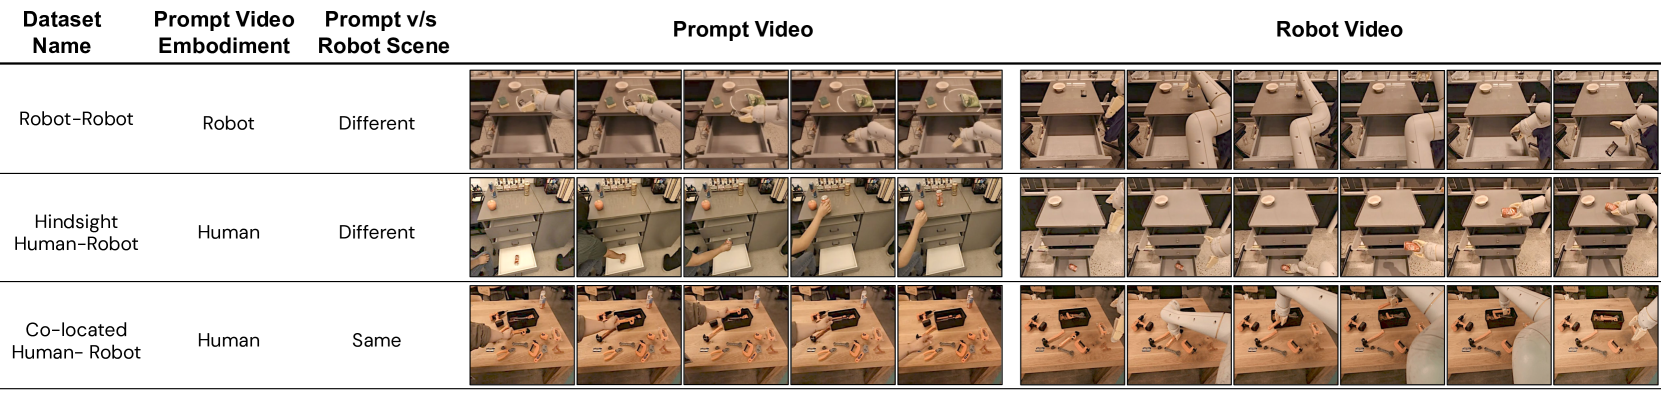
\includegraphics[width=1.0\linewidth]{./chapter8/media/Vid2Robot_Datasets.png}
	\caption[Datasets used to train Vid2Robot]{Datasets used to train Vid2Robot \cite{?}.}
	\label{fig:Vid2RobotDatasets}
\end{figure}
Vid2Robot requires paired prompt videos and robot trajectories performing the same task and is trained with three different dataset categories, see Figure~\ref{fig:Vid2RobotDatasets}.

The three datasets are:
\begin{itemize}
    \item \textbf{Robot-Robot:} Dataset with robot prompt videos and robot trajectories performing the same task. 
    
    \item \textbf{Hindsight Human-Robot Dataset:} Dataset of human demonstrations of manipulation tasks, which are paired with corresponding robot trajectories that perform the same tasks. The human demonstrations are collected with high variablity, for example using left/right hand, individual motion styles, different speeds, randomized robot camera angles.
  
    \item \textbf{Co-located Human-Robot Dataset:} Dataset of humans and robots performing the same task in the same physical workspace.
\end{itemize}
The training corpus contains approximately 100k robot-robot videos and 10k human-to-robot demonstrations. Over 90 percent of the data are robot-robot pairs, and is collected from public avialable sources.




\subsection{Summary}
Vid2Robot is trained on a large-scale video dataset of human manipulation tasks, allowing it to generalize to a wide range of unseen tasks and environments. 
The experimental results demonstrate that Vid2Robot can successfully perform various manipulation tasks, such as object picking, placing, and tool use, by directly learning from robot or human video demonstrations. 
% This approach significantly reduces the need for manual task specification and allows robots to learn from the rich visual information present in human demonstrations, paving the way for more intuitive and efficient robot learning in real-world scenarios.

\section{Paper - ORION: Vision-based Manipulation from Single Human Video with Open-World Object Graphs}
\section{Paper - Learning an Actionable Discrete Diffusion Policy via Large-Scale Actionless Video Pre-Training}

\section{Paper - Learning Video-Conditioned Policies for Unseen Manipulation Tasks}